% Created by tikzDevice version 0.12 on 2019-01-21 17:17:25
% !TEX encoding = UTF-8 Unicode
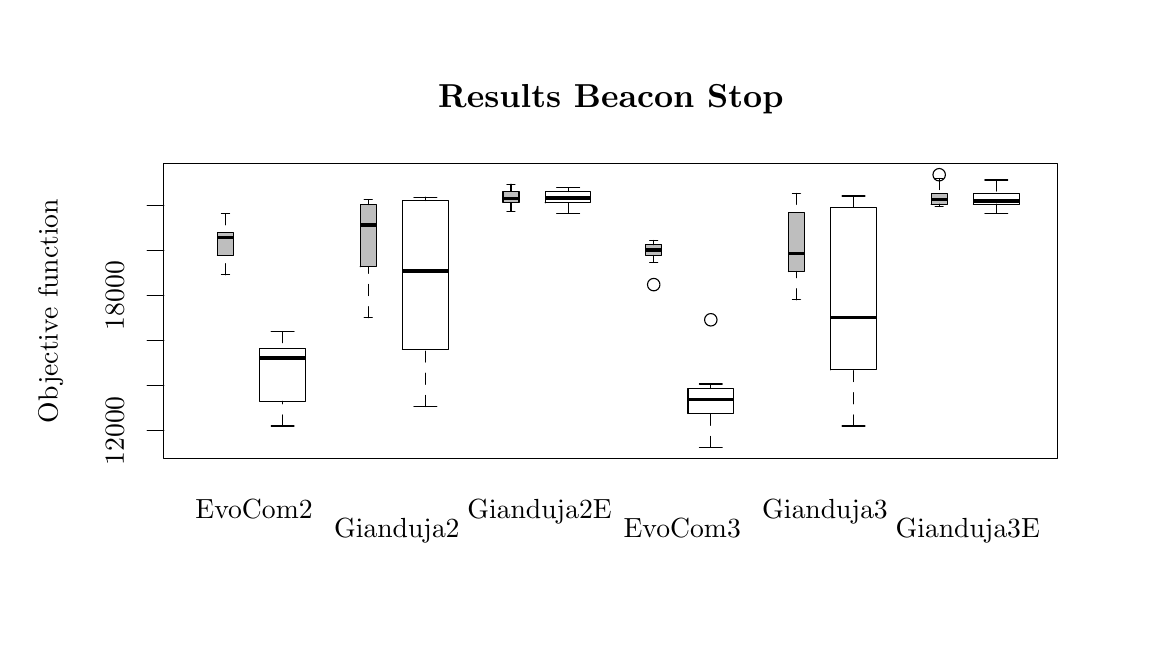
\begin{tikzpicture}[x=1pt,y=1pt]
\definecolor{fillColor}{RGB}{255,255,255}
\path[use as bounding box,fill=fillColor,fill opacity=0.00] (0,0) rectangle (397.48,216.81);
\begin{scope}
\path[clip] ( 49.20, 61.20) rectangle (372.28,167.61);
\definecolor{fillColor}{RGB}{190,190,190}

\path[fill=fillColor] ( 68.59,134.61) --
	( 74.37,134.61) --
	( 74.37,142.72) --
	( 68.59,142.72) --
	cycle;
\definecolor{drawColor}{RGB}{0,0,0}

\path[draw=drawColor,line width= 1.2pt,line join=round] ( 68.59,140.88) -- ( 74.37,140.88);

\path[draw=drawColor,line width= 0.4pt,dash pattern=on 4pt off 4pt ,line join=round,line cap=round] ( 71.48,127.51) -- ( 71.48,134.61);

\path[draw=drawColor,line width= 0.4pt,dash pattern=on 4pt off 4pt ,line join=round,line cap=round] ( 71.48,149.60) -- ( 71.48,142.72);

\path[draw=drawColor,line width= 0.4pt,line join=round,line cap=round] ( 70.04,127.51) -- ( 72.93,127.51);

\path[draw=drawColor,line width= 0.4pt,line join=round,line cap=round] ( 70.04,149.60) -- ( 72.93,149.60);

\path[draw=drawColor,line width= 0.4pt,line join=round,line cap=round] ( 68.59,134.61) --
	( 74.37,134.61) --
	( 74.37,142.72) --
	( 68.59,142.72) --
	( 68.59,134.61);
\definecolor{fillColor}{RGB}{255,255,255}

\path[fill=fillColor] ( 83.86, 81.80) --
	(100.37, 81.80) --
	(100.37,100.75) --
	( 83.86,100.75) --
	cycle;

\path[draw=drawColor,line width= 1.2pt,line join=round] ( 83.86, 97.40) -- (100.37, 97.40);

\path[draw=drawColor,line width= 0.4pt,dash pattern=on 4pt off 4pt ,line join=round,line cap=round] ( 92.11, 72.86) -- ( 92.11, 81.80);

\path[draw=drawColor,line width= 0.4pt,dash pattern=on 4pt off 4pt ,line join=round,line cap=round] ( 92.11,106.97) -- ( 92.11,100.75);

\path[draw=drawColor,line width= 0.4pt,line join=round,line cap=round] ( 87.99, 72.86) -- ( 96.24, 72.86);

\path[draw=drawColor,line width= 0.4pt,line join=round,line cap=round] ( 87.99,106.97) -- ( 96.24,106.97);

\path[draw=drawColor,line width= 0.4pt,line join=round,line cap=round] ( 83.86, 81.80) --
	(100.37, 81.80) --
	(100.37,100.75) --
	( 83.86,100.75) --
	( 83.86, 81.80);
\definecolor{fillColor}{RGB}{190,190,190}

\path[fill=fillColor] (120.17,130.43) --
	(125.95,130.43) --
	(125.95,152.89) --
	(120.17,152.89) --
	cycle;

\path[draw=drawColor,line width= 1.2pt,line join=round] (120.17,145.46) -- (125.95,145.46);

\path[draw=drawColor,line width= 0.4pt,dash pattern=on 4pt off 4pt ,line join=round,line cap=round] (123.06,112.00) -- (123.06,130.43);

\path[draw=drawColor,line width= 0.4pt,dash pattern=on 4pt off 4pt ,line join=round,line cap=round] (123.06,154.66) -- (123.06,152.89);

\path[draw=drawColor,line width= 0.4pt,line join=round,line cap=round] (121.62,112.00) -- (124.50,112.00);

\path[draw=drawColor,line width= 0.4pt,line join=round,line cap=round] (121.62,154.66) -- (124.50,154.66);

\path[draw=drawColor,line width= 0.4pt,line join=round,line cap=round] (120.17,130.43) --
	(125.95,130.43) --
	(125.95,152.89) --
	(120.17,152.89) --
	(120.17,130.43);
\definecolor{fillColor}{RGB}{255,255,255}

\path[fill=fillColor] (135.44,100.61) --
	(151.94,100.61) --
	(151.94,154.37) --
	(135.44,154.37) --
	cycle;

\path[draw=drawColor,line width= 1.2pt,line join=round] (135.44,128.89) -- (151.94,128.89);

\path[draw=drawColor,line width= 0.4pt,dash pattern=on 4pt off 4pt ,line join=round,line cap=round] (143.69, 79.93) -- (143.69,100.61);

\path[draw=drawColor,line width= 0.4pt,dash pattern=on 4pt off 4pt ,line join=round,line cap=round] (143.69,155.53) -- (143.69,154.37);

\path[draw=drawColor,line width= 0.4pt,line join=round,line cap=round] (139.56, 79.93) -- (147.82, 79.93);

\path[draw=drawColor,line width= 0.4pt,line join=round,line cap=round] (139.56,155.53) -- (147.82,155.53);

\path[draw=drawColor,line width= 0.4pt,line join=round,line cap=round] (135.44,100.61) --
	(151.94,100.61) --
	(151.94,154.37) --
	(135.44,154.37) --
	(135.44,100.61);
\definecolor{fillColor}{RGB}{190,190,190}

\path[fill=fillColor] (171.75,153.66) --
	(177.53,153.66) --
	(177.53,157.72) --
	(171.75,157.72) --
	cycle;

\path[draw=drawColor,line width= 1.2pt,line join=round] (171.75,155.03) -- (177.53,155.03);

\path[draw=drawColor,line width= 0.4pt,dash pattern=on 4pt off 4pt ,line join=round,line cap=round] (174.64,150.50) -- (174.64,153.66);

\path[draw=drawColor,line width= 0.4pt,dash pattern=on 4pt off 4pt ,line join=round,line cap=round] (174.64,160.24) -- (174.64,157.72);

\path[draw=drawColor,line width= 0.4pt,line join=round,line cap=round] (173.19,150.50) -- (176.08,150.50);

\path[draw=drawColor,line width= 0.4pt,line join=round,line cap=round] (173.19,160.24) -- (176.08,160.24);

\path[draw=drawColor,line width= 0.4pt,line join=round,line cap=round] (171.75,153.66) --
	(177.53,153.66) --
	(177.53,157.72) --
	(171.75,157.72) --
	(171.75,153.66);
\definecolor{fillColor}{RGB}{255,255,255}

\path[fill=fillColor] (187.02,153.52) --
	(203.52,153.52) --
	(203.52,157.60) --
	(187.02,157.60) --
	cycle;

\path[draw=drawColor,line width= 1.2pt,line join=round] (187.02,155.24) -- (203.52,155.24);

\path[draw=drawColor,line width= 0.4pt,dash pattern=on 4pt off 4pt ,line join=round,line cap=round] (195.27,149.72) -- (195.27,153.52);

\path[draw=drawColor,line width= 0.4pt,dash pattern=on 4pt off 4pt ,line join=round,line cap=round] (195.27,159.01) -- (195.27,157.60);

\path[draw=drawColor,line width= 0.4pt,line join=round,line cap=round] (191.14,149.72) -- (199.40,149.72);

\path[draw=drawColor,line width= 0.4pt,line join=round,line cap=round] (191.14,159.01) -- (199.40,159.01);

\path[draw=drawColor,line width= 0.4pt,line join=round,line cap=round] (187.02,153.52) --
	(203.52,153.52) --
	(203.52,157.60) --
	(187.02,157.60) --
	(187.02,153.52);
\definecolor{fillColor}{RGB}{190,190,190}

\path[fill=fillColor] (223.33,134.51) --
	(229.10,134.51) --
	(229.10,138.38) --
	(223.33,138.38) --
	cycle;

\path[draw=drawColor,line width= 1.2pt,line join=round] (223.33,136.46) -- (229.10,136.46);

\path[draw=drawColor,line width= 0.4pt,dash pattern=on 4pt off 4pt ,line join=round,line cap=round] (226.22,132.07) -- (226.22,134.51);

\path[draw=drawColor,line width= 0.4pt,dash pattern=on 4pt off 4pt ,line join=round,line cap=round] (226.22,139.91) -- (226.22,138.38);

\path[draw=drawColor,line width= 0.4pt,line join=round,line cap=round] (224.77,132.07) -- (227.66,132.07);

\path[draw=drawColor,line width= 0.4pt,line join=round,line cap=round] (224.77,139.91) -- (227.66,139.91);

\path[draw=drawColor,line width= 0.4pt,line join=round,line cap=round] (223.33,134.51) --
	(229.10,134.51) --
	(229.10,138.38) --
	(223.33,138.38) --
	(223.33,134.51);

\path[draw=drawColor,line width= 0.4pt,line join=round,line cap=round] (226.22,123.96) circle (  2.25);
\definecolor{fillColor}{RGB}{255,255,255}

\path[fill=fillColor] (238.59, 77.38) --
	(255.10, 77.38) --
	(255.10, 86.38) --
	(238.59, 86.38) --
	cycle;

\path[draw=drawColor,line width= 1.2pt,line join=round] (238.59, 82.44) -- (255.10, 82.44);

\path[draw=drawColor,line width= 0.4pt,dash pattern=on 4pt off 4pt ,line join=round,line cap=round] (246.85, 65.14) -- (246.85, 77.38);

\path[draw=drawColor,line width= 0.4pt,dash pattern=on 4pt off 4pt ,line join=round,line cap=round] (246.85, 88.06) -- (246.85, 86.38);

\path[draw=drawColor,line width= 0.4pt,line join=round,line cap=round] (242.72, 65.14) -- (250.97, 65.14);

\path[draw=drawColor,line width= 0.4pt,line join=round,line cap=round] (242.72, 88.06) -- (250.97, 88.06);

\path[draw=drawColor,line width= 0.4pt,line join=round,line cap=round] (238.59, 77.38) --
	(255.10, 77.38) --
	(255.10, 86.38) --
	(238.59, 86.38) --
	(238.59, 77.38);

\path[draw=drawColor,line width= 0.4pt,line join=round,line cap=round] (246.85,111.25) circle (  2.25);
\definecolor{fillColor}{RGB}{190,190,190}

\path[fill=fillColor] (274.91,128.69) --
	(280.68,128.69) --
	(280.68,149.91) --
	(274.91,149.91) --
	cycle;

\path[draw=drawColor,line width= 1.2pt,line join=round] (274.91,135.19) -- (280.68,135.19);

\path[draw=drawColor,line width= 0.4pt,dash pattern=on 4pt off 4pt ,line join=round,line cap=round] (277.79,118.46) -- (277.79,128.69);

\path[draw=drawColor,line width= 0.4pt,dash pattern=on 4pt off 4pt ,line join=round,line cap=round] (277.79,156.93) -- (277.79,149.91);

\path[draw=drawColor,line width= 0.4pt,line join=round,line cap=round] (276.35,118.46) -- (279.24,118.46);

\path[draw=drawColor,line width= 0.4pt,line join=round,line cap=round] (276.35,156.93) -- (279.24,156.93);

\path[draw=drawColor,line width= 0.4pt,line join=round,line cap=round] (274.91,128.69) --
	(280.68,128.69) --
	(280.68,149.91) --
	(274.91,149.91) --
	(274.91,128.69);
\definecolor{fillColor}{RGB}{255,255,255}

\path[fill=fillColor] (290.17, 93.20) --
	(306.68, 93.20) --
	(306.68,151.74) --
	(290.17,151.74) --
	cycle;

\path[draw=drawColor,line width= 1.2pt,line join=round] (290.17,112.11) -- (306.68,112.11);

\path[draw=drawColor,line width= 0.4pt,dash pattern=on 4pt off 4pt ,line join=round,line cap=round] (298.43, 72.89) -- (298.43, 93.20);

\path[draw=drawColor,line width= 0.4pt,dash pattern=on 4pt off 4pt ,line join=round,line cap=round] (298.43,155.98) -- (298.43,151.74);

\path[draw=drawColor,line width= 0.4pt,line join=round,line cap=round] (294.30, 72.89) -- (302.55, 72.89);

\path[draw=drawColor,line width= 0.4pt,line join=round,line cap=round] (294.30,155.98) -- (302.55,155.98);

\path[draw=drawColor,line width= 0.4pt,line join=round,line cap=round] (290.17, 93.20) --
	(306.68, 93.20) --
	(306.68,151.74) --
	(290.17,151.74) --
	(290.17, 93.20);
\definecolor{fillColor}{RGB}{190,190,190}

\path[fill=fillColor] (326.48,153.05) --
	(332.26,153.05) --
	(332.26,156.89) --
	(326.48,156.89) --
	cycle;

\path[draw=drawColor,line width= 1.2pt,line join=round] (326.48,154.73) -- (332.26,154.73);

\path[draw=drawColor,line width= 0.4pt,dash pattern=on 4pt off 4pt ,line join=round,line cap=round] (329.37,152.12) -- (329.37,153.05);

\path[draw=drawColor,line width= 0.4pt,dash pattern=on 4pt off 4pt ,line join=round,line cap=round] (329.37,162.31) -- (329.37,156.89);

\path[draw=drawColor,line width= 0.4pt,line join=round,line cap=round] (327.93,152.12) -- (330.82,152.12);

\path[draw=drawColor,line width= 0.4pt,line join=round,line cap=round] (327.93,162.31) -- (330.82,162.31);

\path[draw=drawColor,line width= 0.4pt,line join=round,line cap=round] (326.48,153.05) --
	(332.26,153.05) --
	(332.26,156.89) --
	(326.48,156.89) --
	(326.48,153.05);

\path[draw=drawColor,line width= 0.4pt,line join=round,line cap=round] (329.37,163.67) circle (  2.25);
\definecolor{fillColor}{RGB}{255,255,255}

\path[fill=fillColor] (341.75,153.07) --
	(358.26,153.07) --
	(358.26,156.77) --
	(341.75,156.77) --
	cycle;

\path[draw=drawColor,line width= 1.2pt,line join=round] (341.75,154.19) -- (358.26,154.19);

\path[draw=drawColor,line width= 0.4pt,dash pattern=on 4pt off 4pt ,line join=round,line cap=round] (350.00,149.69) -- (350.00,153.07);

\path[draw=drawColor,line width= 0.4pt,dash pattern=on 4pt off 4pt ,line join=round,line cap=round] (350.00,161.76) -- (350.00,156.77);

\path[draw=drawColor,line width= 0.4pt,line join=round,line cap=round] (345.88,149.69) -- (354.13,149.69);

\path[draw=drawColor,line width= 0.4pt,line join=round,line cap=round] (345.88,161.76) -- (354.13,161.76);

\path[draw=drawColor,line width= 0.4pt,line join=round,line cap=round] (341.75,153.07) --
	(358.26,153.07) --
	(358.26,156.77) --
	(341.75,156.77) --
	(341.75,153.07);
\end{scope}
\begin{scope}
\path[clip] (  0.00,  0.00) rectangle (397.48,216.81);
\definecolor{drawColor}{RGB}{0,0,0}

\node[text=drawColor,rotate= 90.00,anchor=base,inner sep=0pt, outer sep=0pt, scale=  1.00] at ( 10.80,114.41) {Objective function};
\end{scope}
\begin{scope}
\path[clip] (  0.00,  0.00) rectangle (397.48,216.81);
\definecolor{drawColor}{RGB}{0,0,0}

\node[text=drawColor,anchor=base,inner sep=0pt, outer sep=0pt, scale=  1.00] at ( 81.80, 39.60) {EvoCom2};

\node[text=drawColor,anchor=base,inner sep=0pt, outer sep=0pt, scale=  1.00] at (184.95, 39.60) {Gianduja2E};

\node[text=drawColor,anchor=base,inner sep=0pt, outer sep=0pt, scale=  1.00] at (288.11, 39.60) {Gianduja3};

\node[text=drawColor,anchor=base,inner sep=0pt, outer sep=0pt, scale=  1.00] at (133.38, 32.71) {Gianduja2};

\node[text=drawColor,anchor=base,inner sep=0pt, outer sep=0pt, scale=  1.00] at (236.53, 32.71) {EvoCom3};

\node[text=drawColor,anchor=base,inner sep=0pt, outer sep=0pt, scale=  1.00] at (339.69, 32.71) {Gianduja3E};
\end{scope}
\begin{scope}
\path[clip] (  0.00,  0.00) rectangle (397.48,216.81);
\definecolor{drawColor}{RGB}{0,0,0}

\node[text=drawColor,anchor=base,inner sep=0pt, outer sep=0pt, scale=  1.20] at (210.74,188.07) {\bfseries Results Beacon Stop};
\end{scope}
\begin{scope}
\path[clip] (  0.00,  0.00) rectangle (397.48,216.81);
\definecolor{drawColor}{RGB}{0,0,0}

\path[draw=drawColor,line width= 0.4pt,line join=round,line cap=round] ( 49.20, 71.13) -- ( 49.20,152.66);

\path[draw=drawColor,line width= 0.4pt,line join=round,line cap=round] ( 49.20, 71.13) -- ( 43.20, 71.13);

\path[draw=drawColor,line width= 0.4pt,line join=round,line cap=round] ( 49.20, 87.44) -- ( 43.20, 87.44);

\path[draw=drawColor,line width= 0.4pt,line join=round,line cap=round] ( 49.20,103.75) -- ( 43.20,103.75);

\path[draw=drawColor,line width= 0.4pt,line join=round,line cap=round] ( 49.20,120.05) -- ( 43.20,120.05);

\path[draw=drawColor,line width= 0.4pt,line join=round,line cap=round] ( 49.20,136.36) -- ( 43.20,136.36);

\path[draw=drawColor,line width= 0.4pt,line join=round,line cap=round] ( 49.20,152.66) -- ( 43.20,152.66);

\node[text=drawColor,rotate= 90.00,anchor=base,inner sep=0pt, outer sep=0pt, scale=  1.00] at ( 34.80, 71.13) {12000};

\node[text=drawColor,rotate= 90.00,anchor=base,inner sep=0pt, outer sep=0pt, scale=  1.00] at ( 34.80,120.05) {18000};

\path[draw=drawColor,line width= 0.4pt,line join=round,line cap=round] ( 49.20, 61.20) --
	(372.28, 61.20) --
	(372.28,167.61) --
	( 49.20,167.61) --
	( 49.20, 61.20);
\end{scope}
\end{tikzpicture}
